%------------------------------------------------------------------------------------
\section{Heat Flow Preprocessor}

The preprocessor is used for drawing the problems geometry, defining
materials, and defining boundary conditions. The process of construction of heat
flow problems is mechanically nearly identical to the construction of
magnetics problems--refer to Sections~\ref{pencil} through~\ref{coffee} for
an overview of the FEMM editing and problem creation commands. This section
considers those parts of problem definition that are unique to heat flow problems.

\subsection{Problem Definition}

The definition of problem type is specified by choosing the
\texttt{Problem} selection off of the main menu. Selecting this
option brings up the Problem Definition dialog, shown in
Figure~\ref{hfig5}.

\begin{figure}[htbp]
\centerline{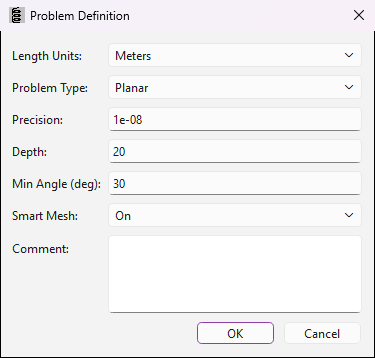
\includegraphics[scale=\dlgscale,max width=\textwidth]{hprobdef}}
\caption{Problem Definition dialog.}
\label{hfig5}
\end{figure}

The dialog's entries, in the order they appear:

\begin{itemize}

\item{\tt Length Units}. This box identifies
what unit is associated with the dimensions prescribed in the
model's geometry. Currently, the program supports inches,
millimeters, centimeters, meters, mils, and $\mu $meters.

\item{\tt Problem Type}. This
drop box allows the user to choose from a 2-D planar problem (the
\texttt{Planar} selection), or an axisymmetric problem (the
\texttt{Axisymmetric} selection).

\item{\tt Precision}. The
number in this edit box specifies the stopping criteria for the
linear solver. The linear algebra problem could be represented by:

\begin{displaymath}
M x = b
\end{displaymath}

\noindent
where $M$ is a square matrix, $b$ is a vector, and $x$ is a vector of
unknowns to be determined. The solver precision value determines the maximum
allowable value for $\vert \vert b - Mx\vert \vert / \vert \vert b\vert
\vert $. The default value is $10^{ - 8}$.

\item{\tt Depth}. If a Planar
problem is selected, this edit box becomes enabled. This value is
the length of the geometry in the ``into the page'' direction. This
value is used for scaling integral results in the post processor
(e.g. force, inductance, etc.) to the appropriate length. The units
of the Depth selection are the same as the selected length units.

\item{\tt Min Angle (deg)}.  The entry in this box is used as a
constraint sent to the mesh generator, {\tt tangle}.  The mesh generator
adds points to the mesh to
ensure that no angles smaller than the specified angle occur. If the minimum angle
is 20.7 degrees or smaller, the triangulation algorithm is theoretically guaranteed to
terminate (assuming infinite precision arithmetic -- the mesh generator may
fail to terminate if you run out of precision).  In practice, the
algorithm often succeeds for minimum angles up to 33.8 degrees.
For highly refined meshes, however, it may be necessary to reduce
the minimum angle to well below 20 to avoid problems associated
with insufficient floating-point precision.  The edit box will accept
values between 1 and 33.8 degrees.

\item{\tt Smart Mesh}.  When {\tt On}, the mesh generator derives a
characteristic element size from the average length of the model's line
segments and applies it at the ends of those segments, refining the mesh
toward corners.  Endpoints belonging only to arcs are left alone, so a
smooth surface is not refined merely for being curved.
When {\tt Off}, element sizes come only from the mesh size specified on each
block label, together with any per-segment maximum side length.

\item{\tt Comment}. The user
can enter in a few lines of text that give a brief description of
the problem that is being solved. This is useful if the user is
running several small variations on a given geometry. The comment
can then be used to identify the relevant features for a particular
geometry.

\end{itemize}

\subsection{Definition of Properties}

To make a solvable problem definition, the user must identify boundary
conditions, block materials properties, and so on. The different types of
properties defined for a given problem are defined via the
\texttt{Properties} selection off of the main menu.

When the \texttt{Properties} selection is chosen, a drop menu
appears that has selections for Materials, Boundary, Point, and
Conductors. When any one of these selections is chosen, the dialog
pictured in Figure~\ref{hfig7} appears.

\begin{figure}[htbp]
\centerline{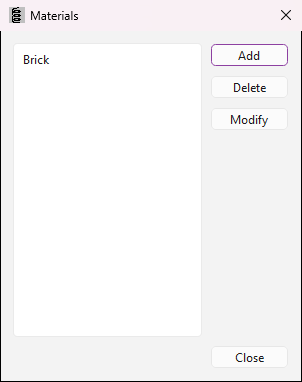
\includegraphics[scale=\dlgscale,max width=\textwidth]{hpropdef}}
\caption{Materials dialog.}
\label{hfig7}
\end{figure}




This dialog is the manager for a particular type of property, and its
title changes to match the type chosen from the menu. All currently
defined properties of that type are listed in the box on the left. At the
beginning of a new model definition, the list will be empty, since no
properties have yet been defined. Pushing the {\tt Add} button allows the
user to define a new property. The {\tt Delete} button removes the
property currently selected in the list, and {\tt Modify} opens the
selected property for viewing and editing --- as does double-clicking the
property itself. {\tt Close} dismisses the dialog. Specifics for defining
the various property types are addressed in the following subsections.

\subsubsection{Point Properties}

If a new point property is added or an existing point property modified, the
\texttt{Nodal Property} dialog box appears. This dialog box is pictured in
Figure~\ref{hfig8}.

\begin{figure}[htbp]
\centerline{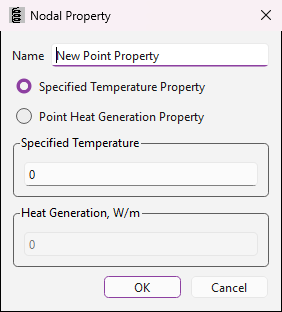
\includegraphics[scale=\dlgscale,max width=\textwidth]{hnodeprop}}
\caption{Nodal Property dialog.}
\label{hfig8}
\end{figure}

The first selection is the \texttt{Name} edit box. The default name
is {\tt New Point Property}, but this name should be changed to
something that describes the property that you are defining.

Next are edit boxes for defining the temperature at a given point, or
prescribing a heat generation at a given point. The type of point
property is chosen via the radio buttons, and the value is entered in the
enabled edit box.

\subsubsection{Boundary Properties}

The \texttt{Boundary Properties} dialog box is used to specify the
properties of line segments or arc segments that are to be
boundaries of the solution domain. When a new boundary property is
added or an existing property modified, the \texttt{Boundary
Property} dialog pictured in Figure~\ref{hfig9} appears.

\begin{figure}[htbp]
\centerline{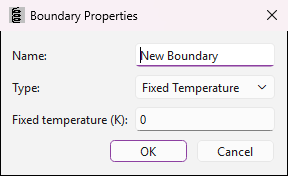
\includegraphics[scale=\dlgscale,max width=\textwidth]{hbdryprop}}
\caption{Boundary Properties dialog.}
\label{hfig9}
\end{figure}

The first selection in the dialog is the \texttt{Name} of the
property. The default name is {\tt New Boundary}, but you should
change this name to something more descriptive of the boundary that
is being defined.

The next selection is the \texttt{Type} drop list. This
specifies the boundary condition type, and the dialog shows only the
parameters that belong to the selected type. Currently, FEMM heat flow
problems support the following types of boundaries: Fixed Temperature,
Heat Flux, Convection, Radiation, Periodic, and Anti-Periodic. These boundary conditions are
described in detail in Section~\ref{bcsection}.

\subsubsection{Materials Properties}

The \texttt{Material Properties} dialog box is used to specify the
properties to be associated with block labels. The properties
specified in this dialog have to do with the material of which the
block is composed. When a new material property is added or an
existing property modified, the
\texttt{Material Properties} dialog pictured in Figure~\ref{hfig10} appears.

\begin{figure}[htbp]
\centerline{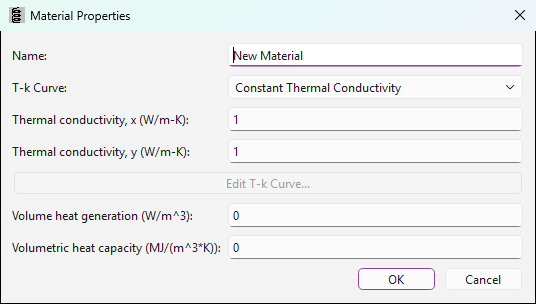
\includegraphics[scale=\dlgscale,max width=\textwidth]{hblockprop}}
\caption{Material Properties dialog.}
\label{hfig10}
\end{figure}

As with Point and Boundary properties, the first step is to choose a
descriptive name for the material that is being described. Enter it in the
\texttt{Name} edit box in lieu of {\tt New Material}.

Next, the thermal conductivity for the material needs to be specified.  The
{\tt T-k Curve} drop list chooses between a conductivity that is constant and
one that varies with temperature.

With {\tt Constant Thermal Conductivity} selected, FEMM
allows you to specify different conductivities in the vertical and horizontal
directions: $k_x$, in the {\tt Thermal conductivity, x} box, applies in the
x- or horizontal direction, and $k_y$, in the
{\tt Thermal conductivity, y} box, in the y- or vertical direction.  Both are
in W/m-K.

If {\tt Thermal Conductivity Depends on Temperature} is selected instead,
those two boxes are disabled and the {\tt Edit T-k Curve...} button becomes
enabled.  Press the button to enter temperature-conductivity pairs, one per
line, in the dialog pictured in Figure~\ref{hfig10b} --- the same
arrangement in which B-H data is entered for a nonlinear magnetic material.
The points need not be entered in order; they are sorted by temperature.
The program interpolates linearly between the entered points, and if it must
extrapolate off the end of the defined curve, conductivity takes the value of
the nearest defined T-k point.  A temperature-dependent material is
isotropic: the interpolated conductivity applies in both directions.

\begin{figure}[htbp]
\centerline{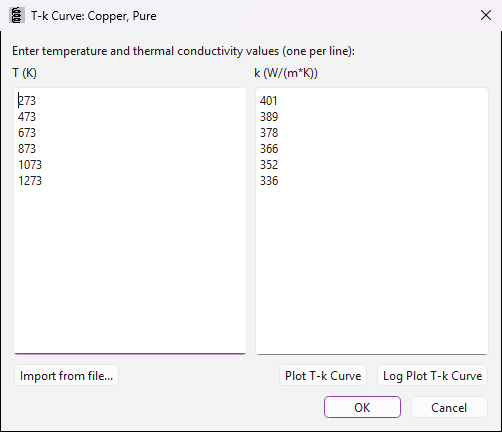
\includegraphics[scale=\dlgscale,max width=\textwidth]{htkdata}}
\caption{Thermal conductivity curve dialog.}
\label{hfig10b}
\end{figure}

The {\tt Import from file...} button reads the points from a two-column text
file.  The program first asks which column is which and what units the file
is in; temperatures in Celsius, Fahrenheit or Rankine and conductivities in
Btu/(ft*hr*F) or kcal/(m*hr*K) are converted to Kelvin and W/(m*K) as they
are read.  {\tt Plot T-k Curve} draws the interpolated curve through the
entered points, so a bad point is easy to spot.

A volume heat generation can also be prescribed, in W/m$^3$, in the
{\tt Volume heat generation} box.

The {\tt Volumetric heat capacity} box, in MJ/(m$^3\cdot$K), is used only by
transient analyses --- that is, by problems that step forward in time from a
previous solution, which are set up through the {\tt hi\_probdef} scripting
command's previous solution and time step arguments.  The entry has no effect
on a steady-state solution.

\subsubsection{Material Library}

Since one kind of material might be needed in several different
models, FEMM has a built-in library of thermal Material Properties definitions.
The user can access and maintain this library through the
\texttt{Properties $\vert $ Material Library} selection off of the
main menu. When this option is selected, the
\texttt{Material Library} dialog pictured in Figure~\ref{hfig11} appears.

\begin{figure}[htbp]
\centerline{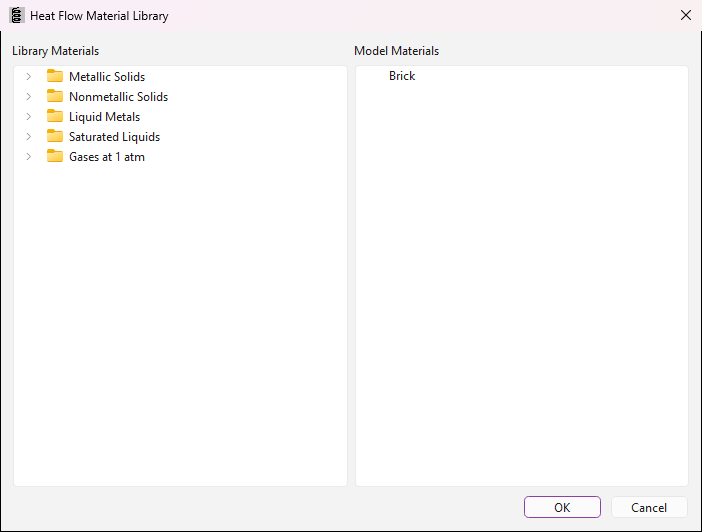
\includegraphics[scale=\dlgscale,max width=\textwidth]{hmatlib}}
\caption{Electrostatics Material Library dialog}
\label{hfig11}
\end{figure}

This dialog allow the user to exchange Block
Property definitions between the current model and the materials
library via a drag-and-drop interface.

A number of different options are available via a mouse button right-click
when the cursor is located on top of a material or folder. Materials can be edited
by double-clicking on the desired material.

Material from other material libraries or models can be imported by selecting the
``Import Materials'' option from the right-button menu that appears when the pointer
is over the root-level folder of either the Library or Model materials lists.

The materials library should be located in the same directory as
the FEMM executable files, under the filename \texttt{heatlib.dat}.
If you move the materials library, FEMM will not be able to find
it.

\subsubsection{Conductor Properties}

The purpose of the conductor properties is mainly to allow the user to apply
constraints on the total amount of heat flowing in and out of a surface.
Alternatively, conductors with a fixed temperature can be defined, and the
program will compute the total heat flow through the during the
solution process.

For fixed temperatures, one could alternatively apply a \texttt{Fixed
Temperature} boundary condition. However, applying a fixed temperature
as a conductor allows the user to group together several physically
disjoint surfaces into one conductor upon which the total heat flux 
is automatically computed.

The dialog for entering conductor properties is pictured in
Figure~\ref{hfig12}.

\begin{figure}[htbp]
\centerline{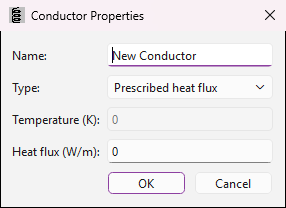
\includegraphics[scale=\dlgscale,max width=\textwidth]{hcircprop}}
\caption{Conductor Properties dialog.}
\label{hfig12}
\end{figure}

The {\tt Name} box names the conductor, so that it can be assigned to
segments and arcs and reported on in the postprocessor.  The {\tt Type}
drop list chooses which of the two quantities is prescribed:
{\tt Prescribed heat flux} or {\tt Prescribed temperature}.  Whichever is selected, its
edit box is enabled and the other is greyed out --- the greyed quantity is
the one the program computes for you during the solution.


\subsection{Analysis Tasks}

Meshing the model, analyzing the model, and viewing the results are
most easily performed by the toolbar buttons pictured in
Figure~\ref{hfig13}.

\begin{figure}[htbp]
\centerline{
\includegraphics{belaman13}}
\caption{Toolbar buttons for starting analysis tasks.}
\label{hfig13}
\end{figure}

The first of these buttons (with the ``yellow mesh'' icon) runs the
mesh generator. The solver actually automatically calls the mesh
generator to make sure that the mesh is up to date, so you never
have to call the mesher from within FEMM. However, it is almost
always important to get a look at the mesh and see that it ``looks
right.'' When the mesh generation button is pressed, the mesher is
called. After the geometry is
triangulated, the finite element mesh is loaded into memory and
displayed underneath the defined nodes, segments, and block labels
as a set of yellow lines.

If you have a very large model, just keeping all of the mesh
information in core can take up a significant amount of memory. If
you are about to analyze a very large problem, it might be a good
idea to choose the \texttt{Mesh $\vert $ Purge Mesh} option off of
the main menu. When this option is selected, the mesh is removed
from memory, and the memory that it occupied is freed for other
uses.

The second button, with the ``hand-crank'' icon, executes the solver,
\texttt{hsolv}. The mesh is brought up to date first: the
\texttt{tangle} mesher is built into the solver, so meshing is the solver's
own first step rather than a separate program. While
hsolv runs, a \texttt{Solver} window displays status information
to the user. hsolv requires no user interaction while it is
running, although the window's \texttt{Abort} button will stop it. When
hsolv is finished analyzing your problem, the window
closes. The time that hsolv requires is highly dependent
on the problem being solved. Solution times are typically on the order of 1
to 10 seconds, depending upon the size and complexity of the problem and the
speed of the machine analyzing the problem.

The ``big magnifying glass'' icon is used to run the postprocessor once the
analysis is finished.



%------------------------------------------------------------------------------------
\section{Heat Flow Postprocessor}

The heat flow postprocessing functionality of FEMM is
used to view solutions generated by the {\tt hsolv} solver.  A heat flow
postprocessor window can be opened either by loading
some previously run analyses via {\tt File|Open} on the main menu,
or by pressing the ``big magnifying glass'' icon from within a
preprocessor window to view a newly generated solution.
Heat flow postprocessor data files stored on disk have the
{\tt .anh} extension.

Operation of the heat flow postprocessor ({\em i.e.} modes, view manipulation) is
very similar to that of the magnetics postprocessor.  Refer to
Sections~\ref{tape} through~\ref{scissors} for this information.

\subsection{Contour Plot}

One of the most useful ways to get a subjective feel for a solution
is by plotting the eqipotentials of temperature. The number and type of equipotential
lines to be plotted can be altered using the Contours Plot icon in
the Graph Mode section of the toolbar (see Figure~\ref{hfig17}). The
Contour Plot icon is the icon with the black contours.

\begin{figure}[htbp]
\centerline{
\includegraphics{hplotbar}}
\caption{Graph Mode toolbar buttons.}
\label{hfig17}
\end{figure}

When this button is pressed, a dialog pops up, allowing the choice of the
number of contours.

\subsection{Density Plot}

Density plots are also a useful way to get a quick feel for the
temperature, flux density, etc., in various parts of the model. By default,
a density plot denoting temperature is displayed when the postprocessor first starts.
(This behavior can be changed via Edit|Preferences on the main menu).
However, the plot can be displayed by pressing the ``spectrum'' button in
the Graph Mode section of the toolbar (see Figure~\ref{hfig17}). A
dialog the pops up that allows the user to turn density plotting
on.

The user can select between density plots of temperature or the magnitude of
temperature gradient or heat flux density. The solution at each
point is classified into one of twenty contours distributed evenly between
either the minimum and maximum flux densities or user-specified bounds.

\subsection{Vector Plots}

A good way of getting a feel for the direction and magnitude of the
field is with plots of the field vectors. With this type of plot
arrows are plotted such that the direction of the arrow indicates
the direction of the field and the size of the arrow indicates the
magnitude of the field. The presence and appearance of this type of
plot can be controlled by pressing the ``arrows'' icon pictured in
Figure~\ref{hfig17}.

\subsection{Line Plots}

When the postprocessor is in Contours Mode, various field values of
interest can be plotted along the defined contour. A plot of a
field value defined contour is performed by pressing the ``graphed
function'' icon in the Plot, Integration and Conductor Results group of toolbar
buttons, shown in Figure~\ref{hfig18}.

\begin{figure}[htbp]
\centerline{
\includegraphics{hresbar}}
\caption{Line Plot, Integration, and Conductor Results toolbar buttons.}
\label{hfig18}
\end{figure}

When this button is pressed, the \texttt{X-Y Plot} dialog (see
Figure~\ref{hfig19}) appears with a drop list containing the types
of line plots available. Choose the desired type of plot and press
``OK.''  The dialog also has an edit box for the number of
points to be sampled along the contour.

\begin{figure}[htbp]
\centerline{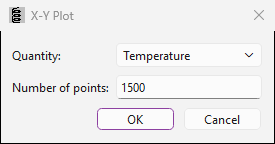
\includegraphics[scale=\dlgscale,max width=\textwidth]{hpltdlg}}
\caption{X-Y Plot dialog.}
\label{hfig19}
\end{figure}

After ``OK'' is pressed, the program computes the desired values
along the defined contour. When the computation is finished, a window
will appear with a plot of the selected quantity.

To save the plotted values, press the \texttt{Export...} button on the
plot window. A file selection dialog appears and prompts for the name
of a file to which the data is written. The data is written as
comma-separated values (\texttt{.csv}), with a header row naming the
columns: position along the contour, followed by one column for each
curve on the plot.

Currently, the type of line plots supported are: Temperature along the
contour; Magnitude of the heat flux density along the contour; Component of heat flux
density normal to the contour; Component of heat flux density tangential to the
contour; Magnitude of the temperature gradient along the contour; Component of
temperature gradient normal to the contour; Component of temperature gradient
tangential to the contour;

In all of these plots, the direction of the normal is understood to
be as shown in Figure~\ref{hfig20}. The tangential direction is
understood to be the direction in which the contour was defined.

\begin{figure}[htbp]
\centerline{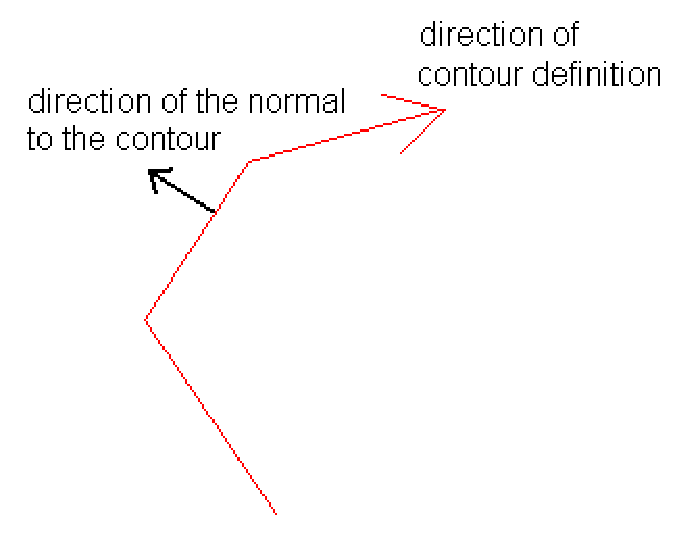
\includegraphics{belaman20}}
\caption{When in doubt plots and integrals taken on this side of a contour.}
\label{hfig20}
\end{figure}




In certain cases, the quantity to be plotted can be ambiguous. This
can occur, for example, if a plot of the tangential field intensity
is requested on a contour running along an interface between two
materials of differing permittivity. In this case, there is a
discontinuity in the tangential field intensity, and the value of
this quantity is different on each side of the interface. The
postprocessor resolves the conflict by always evaluating the plots
at a differentially small distance to the ``normal'' side of the
line. Therefore, by defining the same contour but reversing the
order in which the points are specified, plots of the quantity of
interest on each side of a boundary can be obtained.

\subsection{Line Integrals}

Once a contour has been specified in Contours mode, Line Integrals can be
performed along the specified contour. These integrals are performed by
evaluating a large number of points at evenly spaced along the contour and
integrating using a simple trapezoidal-type integration scheme.

To perform an integration, press the ``integral'' icon on the
toolbar (as shown in Figure~\ref{hfig18}). A small dialog will appear with a
drop list. Choose the desired integral from the drop list and press
\texttt{OK}. The amount of time required to perform the integral
will be virtually instantaneous for some types of integrals;
however, some types may require several seconds to evaluate. When
the evaluation of the integral is completed, the answer appears on
the screen in a pop-up box.

The line integrals currently supported are:


\begin{itemize}


\item \texttt{Temperature Difference (G.t)}. This integral returns the 
temperature difference between the ends of the contour

\item \texttt{Heat Flux (F.n)}. This integral returns the total heat flux passing through
a volume defined by extruding or sweeping the defined contour.

\item \texttt{Contour length \& area}. The length of the contour, and the area formed by
extruding the contour.

\item \texttt{Average temperature}. The average temperature along the line.
\end{itemize}



\subsection{Block Integrals}

To select the regions over which a block integral is to be performed,
left-click with the mouse in the desired region. The selected region will
appear highlighted in green.

To perform an integration, press the ``integral'' icon on the
toolbar (as shown in Figure~\ref{hfig18}), and a dialog will appear
with a drop list. Choose the desired integral from the drop list
and press \texttt{OK}. The integral is then performed by
analytically integrating the specified kernel over each element in
the defined region, and summing the results for all elements.
Volume integrals may take several seconds to evaluate, especially
on dense meshes. Be patient. When the evaluation of the integral is
completed, the answer appears on the screen in a pop-up box.

The block integrals currently supported are:

\begin{itemize}

\item \texttt{Average temperature over volume}

\item \texttt{Block cross-section area}

\item \texttt{Block volume}

\item \texttt{Average F over volume}

\item \texttt{Average G over volume}

\end{itemize}

\subsection{Conductor Results}

If conductor properties are used to specify the excitation, a
useful byproduct is ready access to the temperature of and heat flux through the
conductor. To view the conductor results, either press the ``Conductor Props''
toolbar button pictured in Figure~\ref{hfig18} or select \texttt{View$\vert
$Conductor Properties} off of the postprocessor main menu. A dialog, as
pictured in Figure~\ref{hfig21} will appear. There is a drop list on the
dialog, from which the user selects the conductor for which results
are desired. When a conductor is selected, the temperature and heat flux
associated with that conductor are displayed.

\begin{figure}[htbp]
\centerline{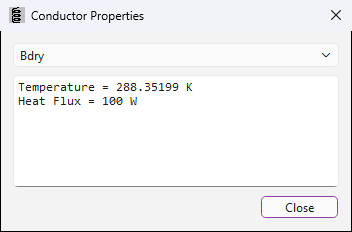
\includegraphics[scale=\dlgscale,max width=\textwidth]{hcircres}}
\caption{Conductor results dialog.}
\label{hfig21}
\end{figure}

